\section{Contexte historique}
    \subsection{La Chine impériale sous la dynastie Qing}

§ Paragraphe 1

Idée :\\
Exemple :\\
Référence :\\
Transition :\\

§ Paragraphe 2

Idée :\\
Exemple :\\
Référence :\\
Transition :\\

§ Paragraphe 3

Idée :\\
Exemple :\\
Référence :\\
Transition :\\

\subsection{La législation chinoise et l’édition des codes légaux}

Les textes de lois chinois relèvent majoritairement du droit pénal et observent une structure définie et rigoureuse. Sous la dynastie des Qing, les codes légaux se divisent en sept chapitres majeurs (appelés \textit{bu}), structure déjà employée pour les textes de lois de la dynastie précédente. En effet, le code des Ming de 1397 utilise cette division en sept chapitres, dont les codes des Qing héritent. Le premier chapitre contient des propos généraux (\og Dénominations et règles \fg \footnote{Les titres de chapitres, entre guillemets, sont empruntés à la traduction proposée par le projet \LSC.}) et les six chapitres suivants sont organisés selon les six ministères (la division du gouvernement en ces six ministères étant observée depuis la dynastie Tang \footnote{Dynastie régnante en Chine de 618 à 907}) : \og Lois administratives \fg, \og Lois domestiques \fg, \og Lois rituelles \fg, etc. À l'instar du code des Ming, ces chapitres sont ensuite divisés en trente sections (en chinois \textit{men}), par exemple \og Institutions administratives \fg, \og Documents officiels \fg, etc. 

Ces chapitres et sections contiennent deux types de lois. Les lois dites principales, les \lu, sont des lois fixes qui constituent la colonne vertébrale du code des Qing (en anglais \textit{statutes}). Certaines lois principales sont directement héritées de la législation de la dynastie Tang, ou ont subi des changements mineurs de vocabulaire. Selon Derk Bodde et Clarence Morris, fixer des lois immuables d'une dynastie à l'autre relèverait d'une vision morale de la loi en Chine : 
\begin{quote}
    No doubt this continuity reflects the Chinese view of law as the codification of moral truths retaining eternal validity irrespective of time or place. \footnote{\cite{law_in_imperial_china}}
\end{quote}

Toutefois, ce propos est nuancé dans leur ouvrage puisque, de fait, moins de la moitié des lois principales demeurent véritablement immuables. Les autres \lu sont modifiées, parfois supprimées ou même créées sous la dynastie Qing, jusqu'en 1740, année de leur dernière version. De plus, les \lu sont accompagnées d'articles additionnels (ou lois secondaires), les \li (aussi appelées \textit{li}, ou en anglais \textit{substatutes}). Les lois secondaires sont des ajouts aux lois principales. Loin d'être figées, elles traitent du droit vivant et viennent préciser la loi principale à laquelle elles sont rattachées. Elles apparaissent souvent à la suite de jugements ou de cas particuliers. Les lois principales ont tendance à se réduire avec le temps. Elles sont au nombre de 436 en 1740. En revanche, les \li augmentent au fur et à mesure. Il en existe une centaine en 1740. À la fin du XIX\ieme siècle, on compte plus de 1 000 lois secondaires. 

 \section{Des sources juridiques}
    \subsection{Les éditions du code légal (1646, 1740)}

Les codes légaux des Qing sont révisés et publiés de manière plus ou moins régulière, tous les dix ans environ. Entre 1740 et 1871, date de la dernière édition du code, on compte 23 rééditions. Toutefois, toutes ces rééditions n'ont pas été conservées, ce qui laisse le corpus incomplet. Dans le cadre du projet \COREL, deux éditions du code légal sont utilisées. 

En 1646, la première édition du code légal des Qing, \dqlj, compte une centaine d'articles. Cette première édition du code s'inscrit dans la continuité du code de la dynastie Ming. Les historiens, notamment Tan Qian  qui a connu les deux dynasties, critiquent cette première édition du code qui n'a pratiquement rien de nouveau et ressemble très fortement au code des Ming. 

La seconde édition du code des Qing intégrée au corpus du projet est le code de 1740, \dq. Dans cette version du code, les \lu sont définitivement établies et ne sont plus modifiées. Comme son nom l'indique, ce texte met sur le même plan les lois principales, \lu et les lois secondaires, \li. En effet, sous la dynastie Ming, les \li n'étaient que des exemples aux lois principales. Elles prennent de plus en plus d'ampleur dans le droit chinois, jusqu'à avoir véritablement la même importance que les lois principales en 1740.

Néanmoins, ces éditions du codes, largement espacées, ne reflètent la loi qu'au moment où elles sont produites et ne prennent pas en compte les modifications qu'il y a pu y avoir entre deux éditions. C'est pourquoi, en plus des éditions des codes légaux, d'autres sources viennent nourrir le projet \COREL : des compilations des textes de lois, qui viennent compléter les zones d'ombres que laissent les codes légaux.

\subsection{Les compilations des textes de loi}

Les compilations des textes de lois sous la dynastie Qing ont une structure similaire à celle des codes légaux et suivent la structure rigoureuse en sept chapitres. Toutefois, ces documents présentent également des caractéristiques qui leur sont propres et viennent compléter les codes légaux. 

En 1871, le \genyuan est publié. Il présente les articles additionnels dans l'ordre chronologique, c'est-à-dire dans l'ordre de modification du code légal. Le \huidian paraît en 1899 et compile l'ensemble des lois en vigueur mais aussi les lois abrogées. Enfin, le \dc est un texte de 1905 qui compile toutes les lois en vigueur sous la dynastie des Qing, avec des explications historiques. Cette compilation a été établie par Xue Yuncheng pour aider à la révision du code légal. Ces trois textes sont des sources qui viennent compléter les textes légaux grâce à leur exhaustivité en présentant toutes les modifications et abrogations des lois et permettent d'en retracer la généalogie.

En plus de ces textes, il existe des recueils de cas qui expliquent l'origine des lois. En effet, les articles additionnels résultent de jugements ou de cas particuliers, il est donc possible de retracer l'origine d'une loi à une affaire, un décret ou un fonctionnaire. Toutefois, ces documents ne font pas partie du projet \COREL. Actuellement en cours de numérisation par la bibliothèque d'études chinoises, les informations supplémentaires que peuvent apporter ces sources constituent une perspective d'enrichissement des données du projet qui sera envisagée à termes. 


\section{Les sources numériques}
    \subsection{Les documents \XML}
Le projet \COREL dispose de sources numériques issues des projets précédents. Ces sources ont été pensées et produites pour deux projets différents et ne sont pas liées entre elles. La source de données principale du projet provient du projet \LSC, qui offre une édition en ligne des sources balisées en \XML. 

\subsubsection{Encodage et validation des données}
Ce balisage \XML relève d'un schéma personnalisé, créé spécifiquement pour le projet \LSC. Pour comprendre ce balisage, il est indispensable de consulter en regard l'édition \XML et le site web du projet, qui sont étroitement liés. En effet, le balisage reprend la structure des codes légaux, familière aux chercheurs, mais lie ce balisage à l'affichage \HTML. Ainsi, certaines portions des textes sont balisées ainsi : 
\begin{minted}{xml}
<p>笞刑五:
    <inf>笞者,擊也,又訓為恥。用小竹板。</inf>一十;
    <inf>折四板。</inf>二十;<inf>除零,折五板。</inf>三十;
    <inf>除零,折一十板。</inf>四十;
    <inf>除零,折一十五板。</inf>五十;
    <inf>折二十板。</inf>
</p>
\end{minted}

En comparant ce code \XML à l'affichage du site, il est possible d'établir clairement le lien entre l'encodage et l'affichage : la balise \texttt{<inf/>} permet d'afficher une partie des paragraphes en caractères bleus, dans une police légèrement inférieure. 
\begin{figure}[h]
    \centering
    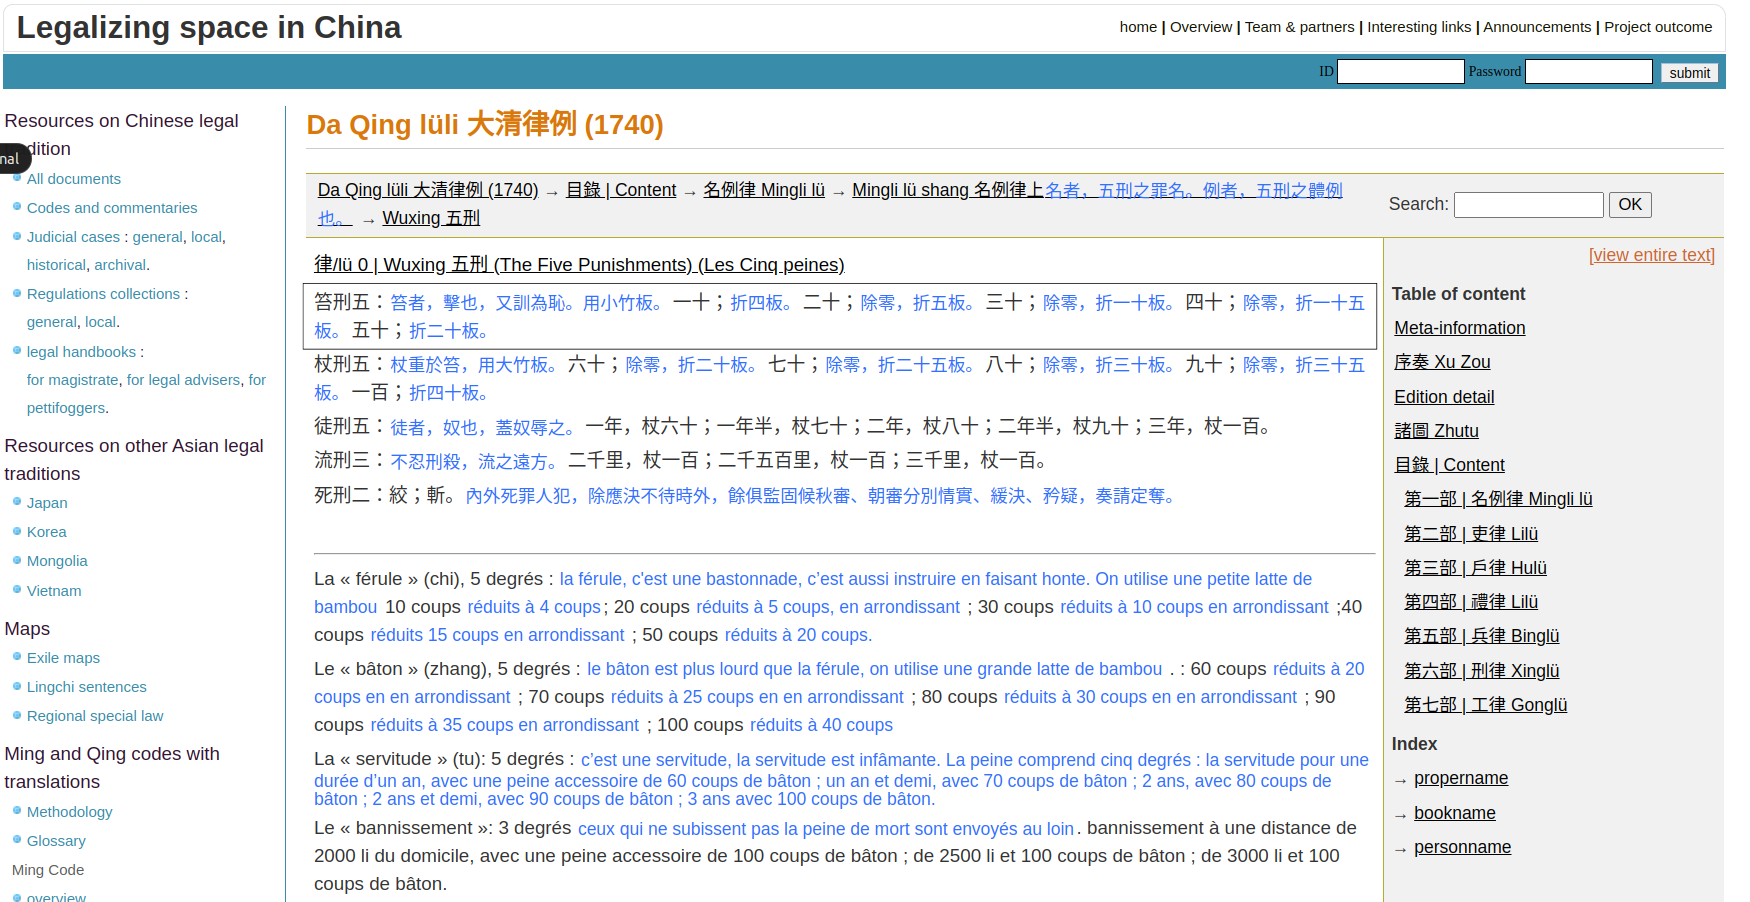
\includegraphics[width=\textwidth]{images/image1.png}
    \caption{Capture d'écran du site web \LSC - affichage du code \XML dans l'encadré.}
    \label{Capture d'écran du site web \LSC}
\end{figure}

Cette utilisation de l'encodage relève du mode de travail des chercheurs sur le projet. En effet, à partir de textes issus de l'OCR, le texte est saisi et balisé dans le logiciel Oxygen au fur et à mesure du projet, c'est-à-dire que l'encodage des données et le développement du site s'effectuent en parallèle. Dès lors, le site web devient un outil de validation de la saisie des données : ce lien entre l'encodage et l'affichage permet aux chercheurs débutants en humanités numériques de vérifier leur code en mettant le site à jour, les erreurs d'affichages se repérant plus facilement qu'un oubli dans le code \XML. 

Mettre en parallèle les étapes d'encodage et de création du site internet relève du choix des chercheurs du projet d'utiliser un schéma \XML entièrement customisé. En effet, ce schéma n'est pas documenté et aucune \DTD n'a été produite pour valider l'encodage et contraindre ce schéma. Le projet \LSC continue aujourd'hui d'être alimenté par les chercheurs du projet \COREL. Dès lors, le seul moyen de se repérer dans un schéma sans documentation ni règles de validation devient l'affichage du site internet.

\subsubsection{Structure des sources numériques}

\subsection{La numérisation des codes légaux}

